\documentclass{article}

\usepackage[utf8]{inputenc}
\usepackage{authblk}
\usepackage{hyperref}
\usepackage[margin=2cm]{geometry}
\usepackage{listings}
\usepackage{graphicx}
\usepackage{subfig}

\lstset{
  language=bash,
  basicstyle=\ttfamily
}

\title{Espotifai\\
\vspace{10pt}
\large Automatic Playlist Recommender}
\author[]{Lucas Emanuel Resck Domingues}
\author[]{Lucas Machado Moschen}

\affil[]{\textit{School of Applied Mathematics}
\\ \textit{Getulio Vargas Foundation}}

\date{\today}

\begin{document}

\maketitle

\begin{center}
    \href{https://github.com/lucasresck/espotifai}{GitHub Repository}
\end{center}

\section{Project statement}

    \textbf{Question}: Which song should we recommend based on
    a playlist and user or context information?

    We can define playlist as a sequence of tracks (audio recordings).
    In this project we aim to study the playlist generation problem, that is,
    given a pool of tracks, a background knowledge about the user,
    and some metadata of songs and playlists, the goal is to create a sequence
    of tracks that satisfies some target as best as possible. The notebooks,
    scripts and work can be found in our repository.

\section{The Datasets}

In order to get user information, we generated a list of usernames in a
networked way.  We visited the Last.fm webpage of several artists and
considered three random users in the top listenings from three different
coutries: Brazil, USA and United Kingdom. Using only these usernames, through
the command \lstinline{generate_lastfm_users.py},  we get additional
Last.fm usernames using the \lstinline{user.getFriends} method from the API. 
With some loops, we can get the network (or part of it). It's possible to have
some bias, unknown yet.

Both databases were built using the Application Programming Interface (API) from the
website, in special
\href{https://developer.spotify.com/documentation/web-api/}{Spotify API} and
\href{https://www.last.fm/api/}{Last.fm API}. Both are great players in the
music business and that was the reason for us to use. 

\subsection{Spotify Database}

We used \href{https://spotipy.readthedocs.io/en/2.13.0/}{Spotipy} Python package
to connect with Spotify's Web API.
It allows us to gather information about public playlists, tracks and artists.
Using the dataset of existing Last.fm users, we sampled a number of users and
tested them to see if they have an account on Spotify. This way, we gathered
information about these users' playlists. Everything that Spotify's API returns
is a \lstinline{.json} file. Playlists data were treated and saved as an
\lstinline{.pkl} file. Each track in the playlists dataset contains an ID, which
identifies the tracks on Spotify and allows us to search for the tracks information.
So we did it, treated the dataset and saved too. Again, we searched for the artists
of the tracks information and what is called \textit{audio features} of the tracks,
that is, a pool of technical metrics like \textit{danceability} (how much a track is
danceable) and \textit{instrumentalness} (how much we are convinced a track is
instrumental). At the end, we have:

\begin{enumerate}
  \item \textbf{Playlists}: Scrapped from users. 11617 playlists, only 6\% duplicated.
  \begin{itemize}
    \item Basic information about a playlist, like its ID, who is the owner, its name.
  \end{itemize}

  \item \textbf{Tracks}: Scrapped from playlists. 849397 tracks, 5\% duplicated, 4.6\% missing.
  \begin{itemize}
    \item Playlist features, like its ID, when the track was added to it, who added it;
    \item Track features, like duration (ms), popularity and name;
    \item Album features, like name and artists (name and ID);
    \item Artists features, like their names and IDS.
  \end{itemize}

  \item \textbf{Audio features}: Scrapped from tracks. No duplicated or missing values.
  \begin{itemize}
    \item A lot of technical features from the audio, like \textit{danceability},
    \textit{energy} and \textit{loudness}. Specially important for the models.
  \end{itemize}

  \item \textbf{Artists}: Scrapped from tracks. Only one artist duplicated.
  \begin{itemize}
    \item Very basic information, like the artist ID and its genres. The genres are
    the most important, because tracks and playlists don't have genres, only the
    artists.
  \end{itemize}
\end{enumerate}

% https://tex.stackexchange.com/a/37583
\begin{figure}%
  \centering
  \subfloat[Distribution of number of tracks among playlists. We can see that most of playlists have few tracks (100 or less), which is reasonable. We also found some outliers, like a playlist that has more than 13000 songs!]{{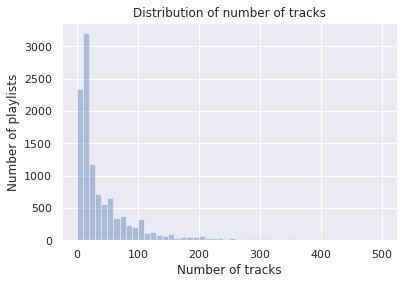
\includegraphics[width=0.3\textwidth]{../../images/sp_number_of_tracks.png} }}%
  \qquad
  \subfloat[Distribution of the duration of a track (in ms). We see that the mode is around 3min20s.]{{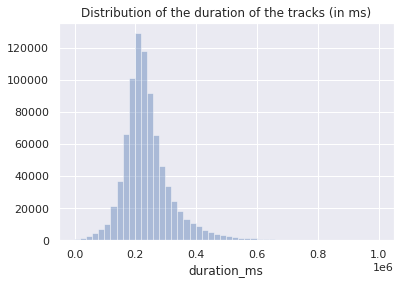
\includegraphics[width=0.3\textwidth]{../../images/sp_duration.png} }}%
  \qquad
  \subfloat[Tracks have artists, and artists have genres. This is the result of our analysis of the genres of the tracks. We see what we would expect: pop, rock, rap and hip hop in the list. The percentages seem small, but there are many genres to consider (in our sample, 2297 genres). This analysis was generated on a sample of the data.]
  {\raisebox{-6ex}%
  {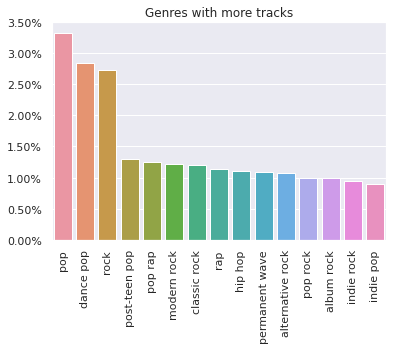
\includegraphics[width=0.3\textwidth]{../../images/sp_genres.png} }}%
  \caption{Visualizations of Spotify data.}%
  \label{fig:example}%
\end{figure}

\subsection{Last.fm Database}

We used \href{https://github.com/pylast/pylast}{pyLast}
package for Python to help with the connection. It organizes all as an object
with several functions. However, in order to retrieve all the information, it
takes a long time to build all datasets: \textbf{Users info}, \textbf{Tracks
info}, \textbf{Artists info} and \textbf{Tags info}, because we retrive a lot
of information in different links from the same API. That's why in the first
analysis we only considered a subset. We got the users randomly from the whole
dataset of users. We saved the information in a \lstinline{json} format. The
variable types were fixed to help the analysis (convertion
\lstinline{string->integer}). The dates were converted to a standart type and
after to datetime. Actually, as we used an API, the data wasn't bad. We
created ids for tracks, tags and artists and save it in a \lstinline{.csv}
file. This structure allow us to save storage. 

The considered datasets were: 

\begin{enumerate}
  \item \textbf{Users}: information about if is subscriber, when he/she 
  has registered, playcounts, country, top artists and tracks and loved
  tracks. The last three are generated by the user and its listening behaviour. (no user had gender, age and number of playlists information and
  we deregarded.) 
  \begin{itemize}
    \item Users: 1000; users with no information: 1.
  \end{itemize}
  \item \textbf{Tracks}: information about reaching, playcounts, duration,
  listeners, similar tracks and top tags.
  \begin{itemize}
    \item tracks: 9902; tracks with no information: 311.
  \end{itemize} 
  \item \textbf{Artists}: information about number of listeners, plays, when
  he/she was published, top tracks, top tags and similar ones.
  \begin{itemize}
    \item artists: 1055; artists with no information: 0.
  \end{itemize}
  \item \textbf{Tags}: information about registration, taggings, reached
  people, top tracks and top artists.
  \begin{itemize}
    \item tags: 1843; tags with no information: 4.
  \end{itemize} 
\end{enumerate}

\begin{figure}[!h]
  \centering
  \label{fig:top-loved}
  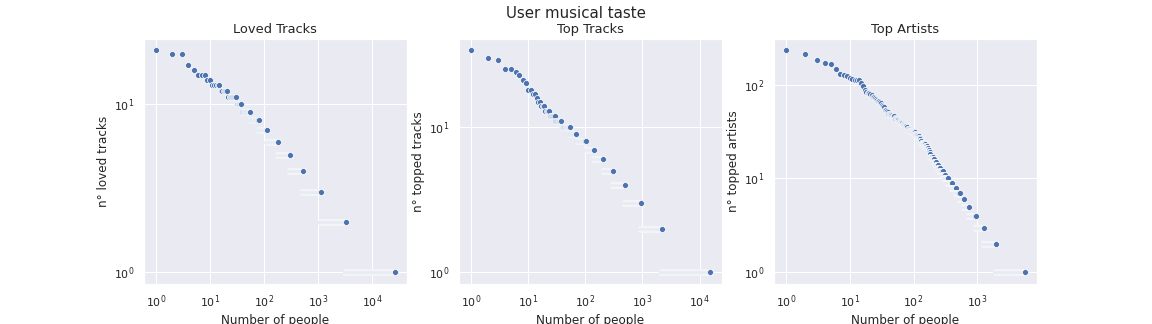
\includegraphics[width = \textwidth]{../../images/top-loved-tracks.png}
  \caption{We can see the distribution of number of top/loved tracks and top artists. All have a Pareto distribution (line in log-log scale; this occurs in other graphics).}
\end{figure}

\section{Gained Insights}

\begin{enumerate}
  \item The distribution of several relations in the data respects a Pareto
  Distribution. It suggests a structure that can be modelled. 
  \item The functions \lstinline{top} and \lstinline{similar} can be useful,
  because it has global information from the Last.fm. 
  \item The dataset from Spotify is the unique with playlist information and
  is the principal for the next work. 
  \item Age and country seems to influenciate less than we thought. Lot of
  missing values.
  \item The distributions of the Spotify audio features are very similar to those
  present on the
  \href{https://developer.spotify.com/documentation/web-api/reference/tracks/get-audio-features/}{Spotify's Web API}.
  It suggests our data is quite representative.
\end{enumerate}

\section{Baseline Model}

It's pretty simple and uses information retrieved from Last.fm. Based on a
playlist (from Spotify), we get all the artists who participate in at least
one song and attribute a weight (number of times it appears in the playlist). After, we get the 200 top artists of the user, weighted by the number of
times the user listened to him/her. With that information, we get the
intersection of the two sets and the correspond weight will be a product of
the normalized weights. If the set is empty, the method does not work, unhappily.
In the intersection set, we take the 10 artists with major weight and for each,
we get his/her 10 top tracks and recommend the $n$ tracks with major weight
(number of playcounts by all the users in the plataform). It uses few information. However, the information is
retrived from a big dataset built by Last.fm and it can be a good baseline to
compare. The first big problem is that it favors artists with well-known
songs. In our example, a playlist with brazilian popular music had all the
recommends with the artist ``Legião Urbana", despite the playlist has a variaty
of artists from Brazil. 

\end{document}